\documentclass[border=3pt]{standalone}
\usepackage{tikz}
\usetikzlibrary{arrows.meta,calc,positioning}
\tikzset{pin/.style={-{Stealth[length=5pt]}},
  blk/.style={draw, thick, minimum width=40mm, minimum height=10mm, font=\sffamily\small, align=left}}
\begin{document}
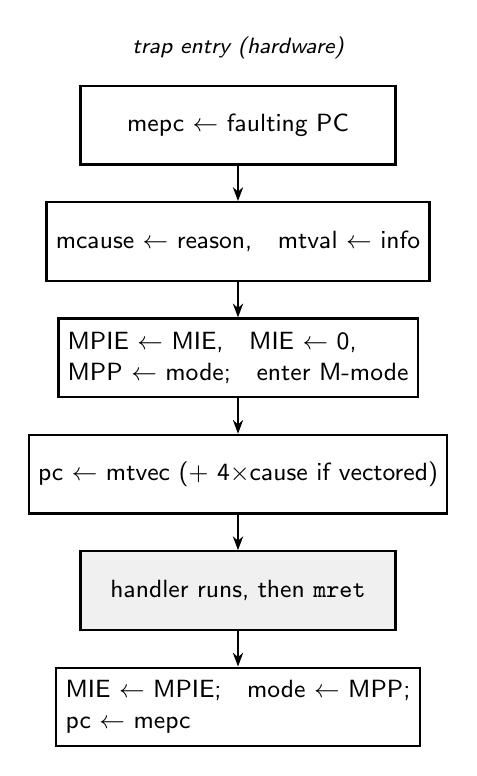
\begin{tikzpicture}[font=\sffamily\small, node distance=4.5mm]
  \node[blk] (t1) at (0,0) {mepc $\leftarrow$ faulting PC};
  \node[blk, below=of t1] (t2) {mcause $\leftarrow$ reason,\quad mtval $\leftarrow$ info};
  \node[blk, below=of t2] (t3) {MPIE $\leftarrow$ MIE,\quad MIE $\leftarrow$ 0,\\MPP $\leftarrow$ mode;\quad enter M-mode};
  \node[blk, below=of t3] (t4) {pc $\leftarrow$ mtvec (+ 4$\times$cause if vectored)};
  \node[blk, below=of t4, fill=black!6] (t5) {handler runs, then \texttt{mret}};
  \node[blk, below=of t5] (t6) {MIE $\leftarrow$ MPIE;\quad mode $\leftarrow$ MPP;\\pc $\leftarrow$ mepc};
  \foreach \a/\b in {t1/t2, t2/t3, t3/t4, t4/t5, t5/t6}{\draw[pin] (\a.south) -- (\b.north);}
  \node[font=\sffamily\footnotesize\itshape, above=2mm of t1.north] {trap entry (hardware)};
\end{tikzpicture}
\end{document}
